% Povinný argument: Kód předmětu
\newcommand{\subject}{MPC-TLS}
% Povinný argument: Název předmětu
\newcommand{\subjectname}{Telekomunikační systémy}
% Povinný argument: Seznam autorů
\newcommand{\authors}{czechbol}
% Povinný argument: Seznam korektorů
\newcommand{\corrections}{kámen u~cesty}
% Nepovinný argument: Popis dokumentu
\newcommand{\docdesc}{Otázky ke~zkoušce}
% Nepovinný argument: Cílová skupina dokumentu
\newcommand{\docgroup}{Informační bezpečnost, FEKT VUT}
% Nepovinný argument: URL repozitáře nebo jiný odkaz na dokument
\newcommand{\docurl}{https://github.com/VUT-FEKT-IBE/WIP-MPC-TLS}

% Přepsáním argumentu na 'false' vypnete balíček 'minted' pro sázení kódu.
% Pro jeho použití lokálně musíte mít v systému dostupný Python 3, python
% knihovnu 'minted' a PDFLaTeX musíte spouštět s argumentem '-shell-escape'.
% Místo něj můžete použít prostředí 'lstlisting'.
\newcommand{\docminted}{false}

% FEKT.tex
% https://github.com/VUT-FEKT-IBE/FEKT.tex
% Git hash repozitáře v době kopírování: 67fb27697810846e93123e0ca293a5107707a854

\documentclass[
    % Velikost základního písma je 12 bodů
    12pt,
    % Formát papíru je A4
    a4paper,
    % Oboustranný tisk
    twoside,
    % Záložky a metainformace ve výsledném PDF budou v kódování unicode
    unicode,
]{article}

%%%%%%%%%%%%%%%%%%%%
% OBECNÉ NASTAVENÍ %
%%%%%%%%%%%%%%%%%%%%

% Kódování zdrojových souborů
\usepackage[utf8]{inputenc}
% Kódování výstupního souboru
\usepackage[T1]{fontenc}
% Podpora češtiny
\usepackage[czech]{babel}

% Geometrie stránky
\usepackage[
    % Horní a dolní okraj
    tmargin=25mm,
    bmargin=25mm,
    % Vnitřní a vnější okraj
    lmargin=30mm,
    rmargin=20mm,
    % Velikost zápatí
    footskip=17mm,
    % Vypnutí záhlaví
    nohead,
]{geometry}

% Zajištění kopírovatelnosti a prohledávanosti vytvořených PDF
\usepackage{cmap}
% Podmínky (pro použití v titulní straně)
\usepackage{ifthen}

%%%%%%%%%%%%%%%
% FORMÁTOVÁNÍ %
%%%%%%%%%%%%%%%

% Nastavení stylu nadpisů
\usepackage{sectsty}
% Formátování obsahů
\usepackage{tocloft}
\setcounter{tocdepth}{1}
% Odstranění mezer mezi řádky v seznamech
\usepackage{enumitem}
\setlist{nosep}
\setitemize{leftmargin=1em}
\setenumerate{leftmargin=1.5em}
\renewcommand{\labelitemi}{--}
\renewcommand{\labelitemii}{--}
\renewcommand{\labelitemiii}{--}
\renewcommand{\labelitemiv}{--}
% Sázení správných uvozovek pomocí '\enquote{}'
\usepackage{csquotes}
% Vynucení umístění poznámek pod čarou vespod stránky
\usepackage[bottom]{footmisc}
% Automatické zarovnání textu k předcházení vdov a parchantů
\usepackage[defaultlines=3,all=true]{nowidow}
% Zalomení části textu pokud není na současné stránce dost místa
\usepackage{needspace}
% Nastavení řádkování
\usepackage{setspace}
\onehalfspacing
% Změna odsazení odstavců
\setlength{\parskip}{1em}
\setlength{\parindent}{0em}

% Bezpatkové sázení nadpisů
\allsectionsfont{\sffamily}
% Změna formátování nadpisu a podnadpisů v Obsahu
\renewcommand{\cfttoctitlefont}{\Large\bfseries\sffamily}
\renewcommand{\cftsubsecdotsep}{\cftdotsep}

% Použití moderní/aktualizované sady písem
\usepackage{lmodern}

%%%%%%%%%%%
% NADPISY %
%%%%%%%%%%%

\usepackage{titlesec}

\titlespacing*{\section}{0pt}{10pt}{-0.2\baselineskip}
\titlespacing*{\subsection}{0pt}{0.2\baselineskip}{-0.2\baselineskip}
\titlespacing*{\subsubsection}{0pt}{0.2\baselineskip}{-0.2\baselineskip}
\titlespacing*{\paragraph}{0pt}{0pt}{1em}

%%%%%%%%%%
% ODKAZY %
%%%%%%%%%%

% Tvorba hypertextových odkazů
\usepackage[
    breaklinks=true,
    hypertexnames=false,
]{hyperref}
% Nastavení barvení odkazů
\hypersetup{
    colorlinks,
    citecolor=black,
    filecolor=black,
    linkcolor=black,
    urlcolor=blue
}

%%%%%%%%%%%%%%%%%%%%%%%%%%%
% OBRÁZKY, GRAFY, TABULKY %
%%%%%%%%%%%%%%%%%%%%%%%%%%%

% Vkládání obrázků
\usepackage{graphicx}
\usepackage{subfig}
% Nastavení popisů obrázků, výpisů a tabulek
\usepackage{caption}
\captionsetup{justification=centering}
% Grafy a vektorové obrázky
\usepackage{tikz}
\usetikzlibrary{shapes,arrows}
% Složitější tabulky
\usepackage{tabularx}
\usepackage{multicol}


\usepackage{wrapfig}
%
\usepackage{float}

% Sázení osamocených float prostředí v horní části stránky
\makeatletter
\setlength{\@fptop}{0pt plus 10pt minus 0pt}
\makeatother

% Vynucení vypsání floating prostředí pomocí \FloatBarrier
\usepackage{placeins}

%%%%%%%%%%%%%%
% MATEMATIKA %
%%%%%%%%%%%%%%

% Sázení matematiky a matematických symbolů ('\mathbb{}')
\usepackage{amsmath}
\usepackage{amssymb}
% Sázení fyzikálních veličin
\usepackage{siunitx}

%%%%%%%%%%%%%%%%%
% ZDROJOVÉ KÓDY %
%%%%%%%%%%%%%%%%%

% Sazba zdrojových kódů
\usepackage[formats]{listings}
% Přepnutí prostředí 'code' do režimu výpisu kódu
\newenvironment{code}{\captionsetup{type=listing}}{}

% Balíček 'minted' budeme používat pouze pokud je jeho hodnota nastavena na 'true'
\providecommand{\docminted}{false}
\ifthenelse{\equal{\docminted}{true}}
{
    % Sazba zdrojových kódů
    \usepackage[newfloat]{minted}
    % Nastavení barev 'minted' kódů
    \usemintedstyle{pastie}
}
{
    % \docminted není 'true', nic neprovádíme
    % Pokud je v dokumentu 'minted' prostředí, dokument se nepodaří přeložit.
}

%%%%%%%%%%%
% TITULKA %
%%%%%%%%%%%

\IfFileExists{./.repo.tex}{
    % Soubor '.repo.tex' může (re)definovat povinné a nepovinné argumenty
    % souboru 'main.tex'. To lze využít v případech kdy v jednom repozitáři
    % existuje více dokumentů najednou (např. státnicové otázky).
    \input{.repo}
}{}

% Pokud byly nepovinné argumenty zakomentovány nebo vymazány, přidáme prázdné
% definice příkazů, aby bylo dokument možné správně přeložit.
\providecommand{\docdesc}{}
\providecommand{\docgroup}{}
\providecommand{\docurl}{}

\newcommand{\titulka}{
    \vspace*{2em}
    \begin{center}
        {\Huge \bfseries \subject}

        \vspace*{1em}

        {\Huge \bfseries \subjectname}

        \vspace*{2em}

        {\Large \docdesc}

        \vspace*{1em}

        \docgroup

        \url{\docurl}
    \end{center}

    \vfill

    \begin{tabular}{ll}
        Text:      & \authors     \\
        Korektura: & \corrections \\
    \end{tabular}
    \hfill
    \today

    \thispagestyle{empty}
    \newpage
}

\clearpage

\newcounter{questionno}
\setcounter{questionno}{0}
\newcommand{\question}[1]{
\addtocounter{questionno}{1}
\thequestionno) \textsf{\large \textbf{#1}}
}

\begin{document}

\pagenumbering{gobble}
\setcounter{page}{0}

\titulka{}

\clearpage

\pagenumbering{arabic}

\section{Vysvětlete pojem konvergované telekomunikace, resp.\ konvergence telekomunikačních sítí.}

\textbf{Konvergence -- (Sbíhavost)}

U 5.\ generace ústředen, sloučení telefonních a IP sítí > IP telefonie, VoIP, paketová telefonie. Není zde účastníkovi trvale vystavěn okruh po dobu hovoru. Hovor je přenášen v malých paketech skrze IP síť.

\section{Vysvětlete pojmy Transwitch, Softswitch+Media gateway. Uveďte některé představitele či platformy, odlišnosti a oblast využití.}

\textbf{Transwitch - HW ústředna}

Uplatnění je univerzální a spolehlivé - koncový zákazníci a poskytovatelé.
Pro spojování je využito specifického HW.\@ Použití zejména pro TDM a výkonné systémy. (Siemens EWSD, Alcatel 1000 S12)

\textbf{Softswitch - SW ústředna} s přidanou funkcionalitou klasické ústředny, zatím pouze menší ústředny. Uplatnění: VoIP, poskytovatele,specifické aplikace-embedded, TMD-VoIP atd.

Můžeme rozdělit dle otevřenosti zdrojového kódu na:
\begin{itemize}[noitemsep]
    \item Open Source (Asterisk, FreeSwitch, YATE, \ldots)
    \item Proprietární (výrobců Alcatel, Panasonic, Siemens, \ldots) \textbf{Media gateway}
\end{itemize}

\noindent MGCP (Media Gateway Control Protocol) je master/slave protokol pro řízení brány (slave).

Standardní komponenty:
\begin{itemize}[noitemsep]
    \item Media Gateway (MG) - brána IP na E1, POTS, ISDN-BRI, PRI porty- Call Agent (CA), Media Gateway Controller (MGC)
    \item textově orientovaný protokol vycházející z HTTP
    \item pro přenos signalizace se používá UDP, nebo TCP
    \item standardní port brány (MG) je 2427
    \item standardní port Call Agenta (CA) je 2727
    \item správa multimediální relace tunelovaným protokolem SDP
    \item real-time multimediální přenos protokolem RTP nebo šifrovaným SRTP, Formát protokolu MGCP je příkaz - odpověď.
\end{itemize}

Příkaz začíná slovem se čtyřmi znaky: AUEP, AUCX, CRCX, DLCX, EPCF, MDCX, NTFY, RQNT, RSIP.\@
Odpověď začíná třemi čísly tzv.\@ kódu odpovědi, např. 200 (OK), podobně jako SIP.\@ V protokolu MGCP má každý příkaz transakční ID, které obsahuje i odpověď.


\newpage

\section{Porovnejte výhody a nevýhody použití Open Source ústředen a proprietárních ústředen, tj. ústředen tradičních výrobců. Uveďte a odůvodněte nejčastější aplikace.}

\begin{figure}[h!]
    \begin{center}
        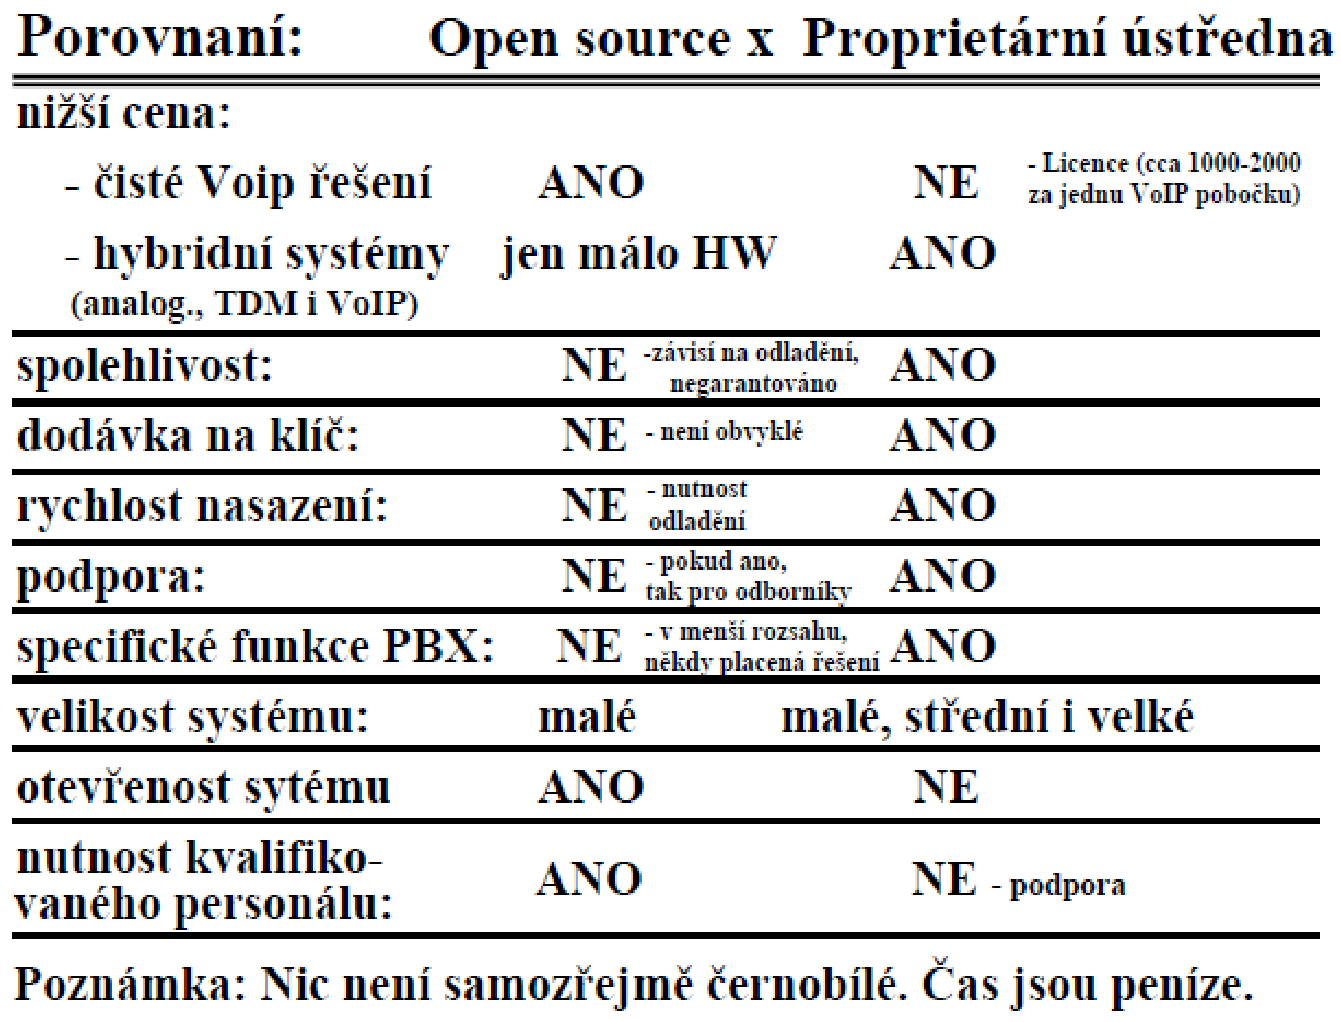
\includegraphics[width=\textwidth]{images/otazka3.png}
        \caption{Srovnání - Open source vs. Proprietary}
        \label{img:1}
    \end{center}
\end{figure}

\noindent Asterisk -- zadarmo, ústředna

\noindent Zoiper -- zadarmo, telefon

\noindent Skype -- zadarmo, telefon, jednoduchá obsluha i lajkem. (WIN)


\newpage

\section{Co je to DID a DISA? Vysvětlete na příkladu PBX v síti s pevným číslovacím plánem. Který typ byste očekávali u menších a který u větších PBX?}

\textbf{DID (DDI):}

Mají li pobočky čísla ve veřejném číslovacím plánu, můžeme volit přímou volbou (DID - Direct Inward Dialing). Číslo pobočky se skládá z čísla ústředny (např. VUT 54114) a čísla pobočky (např. 6990).

\noindent\textbf{DISA:}

Nemají li pobočky PBX vyhrazena čísla ve veřejném číslovacím plánu, můžeme být přepojeni na spojovatelku.

Dnes velmi často využívána interaktivní hlasová odezva IVR (Interactive voice response), která \uv{nasměruje} k další volbě.

Další možností je použití tzv.\ dovolby - doplňková volba (DISA - Direct Inward Subscriber Access).

Po zadání čísla PBX dojde k okamžitému vyzvednutí a dostáváme oznamovací tón PBX (zpravidla konstantní tón, nebo i jiný dle konfigurace).

DISA:\@ oznamovací tón 512 345 678 speciální oznamovací tón 45

DISA-IVR:\@ oznamovací tón 512 345 678 hláška IVR 4 hláška IVR 5

\section{Co je to šetřící automat LCR (ARS)? Vysvětlete funkci. Načrtněte obrázek funkce některé z implementací šetřícího automatu. Co je to normalizace?}

Ústředny obsahají vždy i pokročilejší techniky směrování, označované jako:
\begin{itemize}[noitemsep]
    \item ARS (Automatic Route Selection) Automatická volba směrování
    \item LCR (Low Cost Routing) Šetřící automat
\end{itemize}

\emph{Pozn. Jedná se o totéž. Někteří výrobci používají název ARS, jiní LCR.}

Pobočkové ústředny mají zpravila více vnějších rozhraní a je možné připojení k více poskytovatelům. Pomocí funkce ARS/LCR lze na základě voleného čísla určit nejlevnější cestu nebo i poskytovatele volání. S ohledem na možnost přenositelnosti telefonního čísla se nemusí jednat vždy o nejvhodnější volbu.

Funkce ARS/LCR lze využít i pro směrování příchozích hovorů, v případě tranzitních hovorů.

\noindent Funkce ARS/LCR:
\begin{itemize}[noitemsep]
    \item Vstupní normalizace čísla volaného popř. volajícího.
    \item Vyhledání nejvhodnější cesty směrování hovoru (svazek, svazky) dle:
    \begin{itemize}[noitemsep]
        \item prefixu
        \item času volání
        \item oprávnění pobočky
        \item volných minut svazku, atd.
    \end{itemize}
    \item Výstupní normalizace čísla volaného a volajícího, zahrnující minimálně úpravu čísla pobočky na číslo, pod kterým je dostupná z veřejné sítě.
\end{itemize}

Rozsah možností RS/LCR je dán konkrétní implementací výrobce. V některých PBX lze vytvářet nejen pravidla směrování, ale i definovat sled událostí. Např. po určitém prefixu a obsazení přenašeče generovat oznamovací tón, další čísla pak přímo odesílat na přenašeč atd.


\begin{figure}[h!]
    \begin{center}
        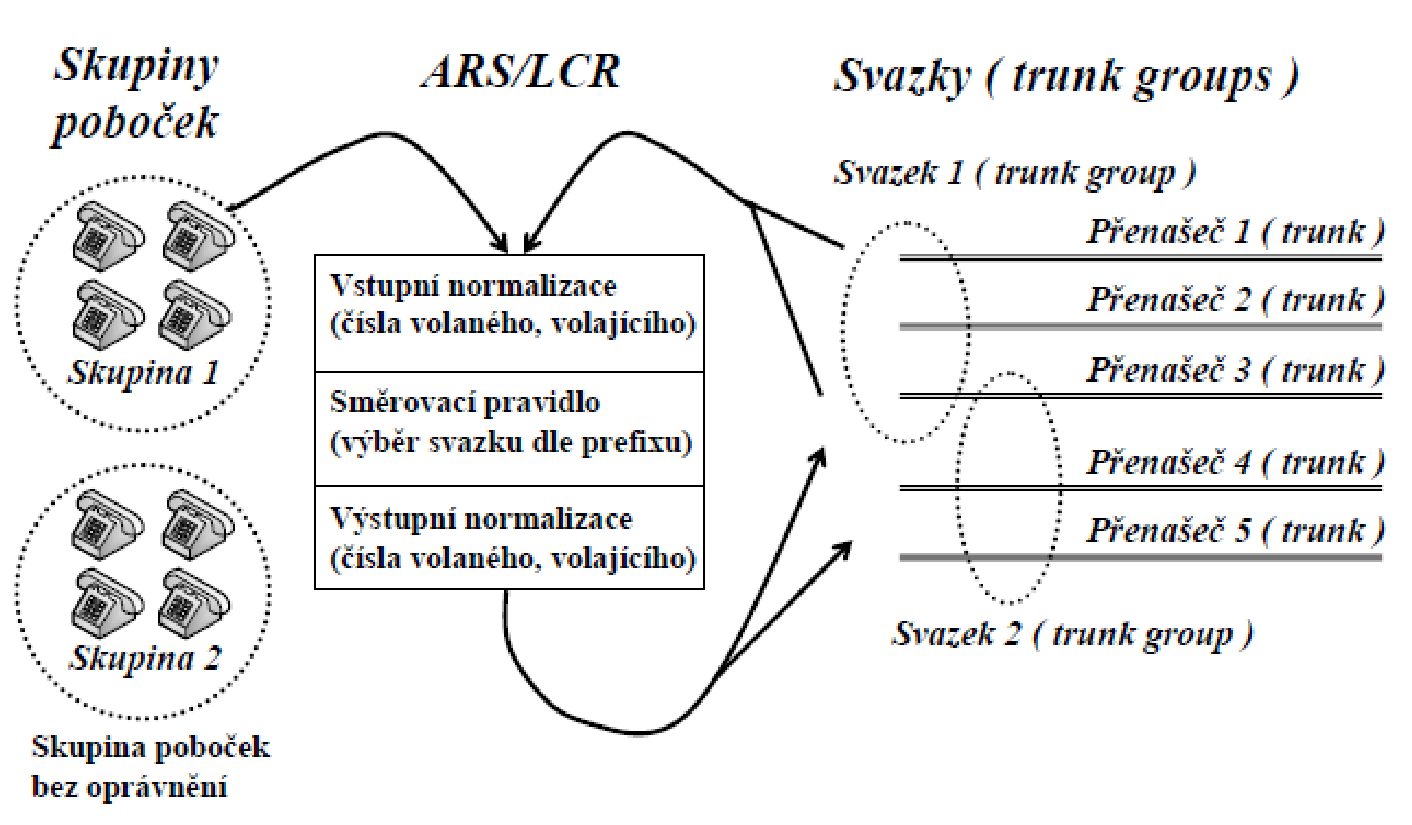
\includegraphics[width=\textwidth]{images/otazka5.png}
        \caption{ARS/LCR}
        \label{img:2}
    \end{center}
\end{figure}

\section{Vysvětlete princip směrování hovorů v PBX Asterisk. K čemu slouží kontexty? Uveďte jednoduchý příklad s pomocí souboru rozhraní a volacího (směrovacího) plánu.}

\begin{figure}[H]
    \begin{center}
        \begin{minipage}[c]{0.35\textwidth}
            Každá pobočka, přenašeč (kanál) je v konfiguračním souboru přidružena kontextu -- context. Směrování je realizováno na základě směrovacích pravidel -- Dialplan, která obsahují souhrn pravidel pro každý kontext. Nejčastěji na základě prefixu volaného čísla je využito pravidlo s nejlepší shodou. Kontexty tak reprezentují skupiny s daným oprávněním.
        \end{minipage}%
        \begin{minipage}[c]{0.65\textwidth}
            \centering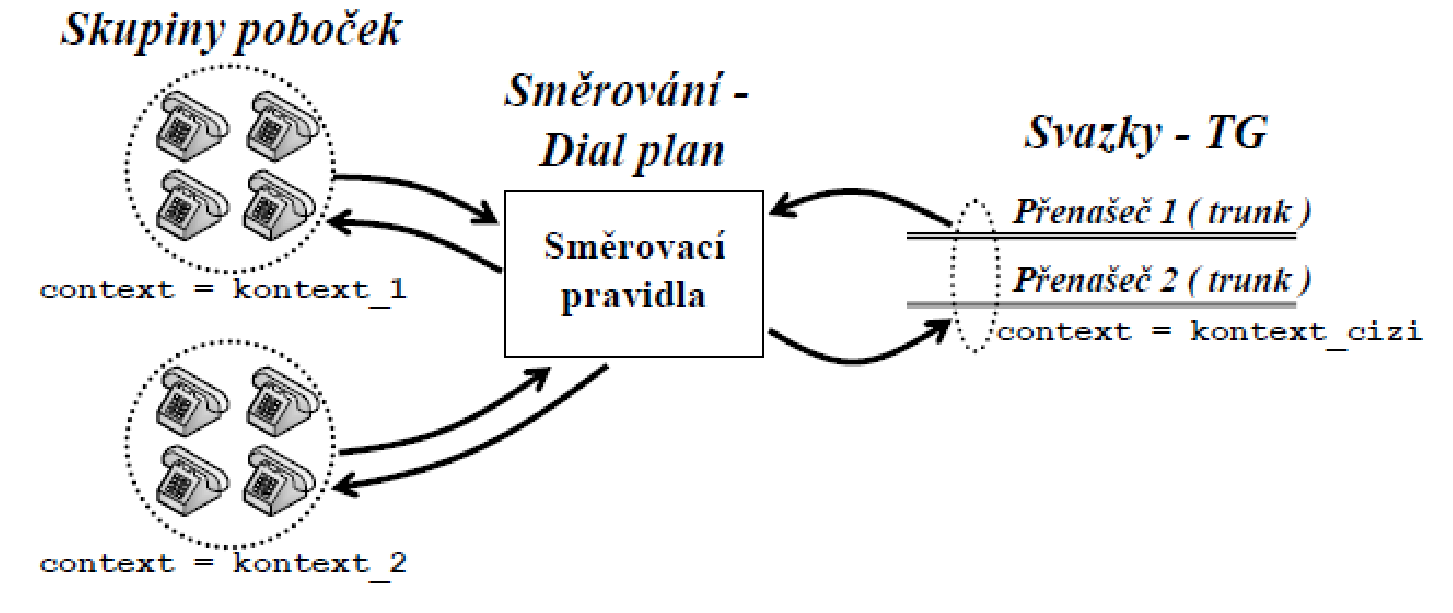
\includegraphics[width=12cm]{images/otazka6.png}
        \end{minipage}
\end{center}
\end{figure}

\section{Charakterizujte Open Source PBX. Pro které aplikace je nutno doplnit specifický HW? Uveďte některé výrobce specifického HW pro Open Source PBX.}

\textbf{Open Source PBX ústředny:}
\begin{itemize}[noitemsep]
    \item Výhradně jsou realizovány jako softswitch.
    \item Využívající otevřeného softwaru a běžného HW.
    \item Pro vazbu na specifická TDM nebo PSTN rozhraní doplněny o telefonní karty či Media Gateway.
    \item Sponzory těchto projektů jsou často výrobci specifického HW pro Open Source softswitche.
    \item Jedná se zatím o spíše o menší systémy, umožňující zpracovat menší počet hovorů. Konkrétní počet je samozřejmě dán výkonností použitého HW, počtem kodeků používaných v systému atd.
    \item Dalším místem využití je i realizace VoIP/TDM bran.
\end{itemize}

\noindent\textbf{Vybraná Open Source PBX řešení:}
\begin{itemize}[noitemsep]
    \item Asterisk > Podporován výrobcem telefonního HW Digium.
    \item FreeSWITCH • YATE
    \item SIP Express Router, a další.
\end{itemize}

\section{Architektura PBX Asterisk. Uveďte základní čtyři API rozhraní a jejich využití. K čemu slouží Dynamic Module Loader, Codec Translator, Application Launcher?}

PBX Switching Core -- přepojovací jádro transparentně spojující příchozí volání na jednotlivých HW a SW rozhraních.

Application Launcher -- spouštěč aplikací zajišťujících např. Hlasovou poštu, přehraní souborů atd.

Codec Translator -- realizuje překódování jednotlivých zvukových kompresních formátů.
Scheduler and I/O Manager -- ovládání rozvrhování nízkoúrovňových úloh a systémového řízení pro dosažení optimálního výkonu del stavu zatížení.

Dynamic Module Loader -- modul, který po startu sytému zavede a inicializuje moduly Asterisk kanálů, souborových formátů, kodeků i aplikací a provede slinkování s interními API rozhraními.

\begin{figure}[h!]
    \begin{center}
        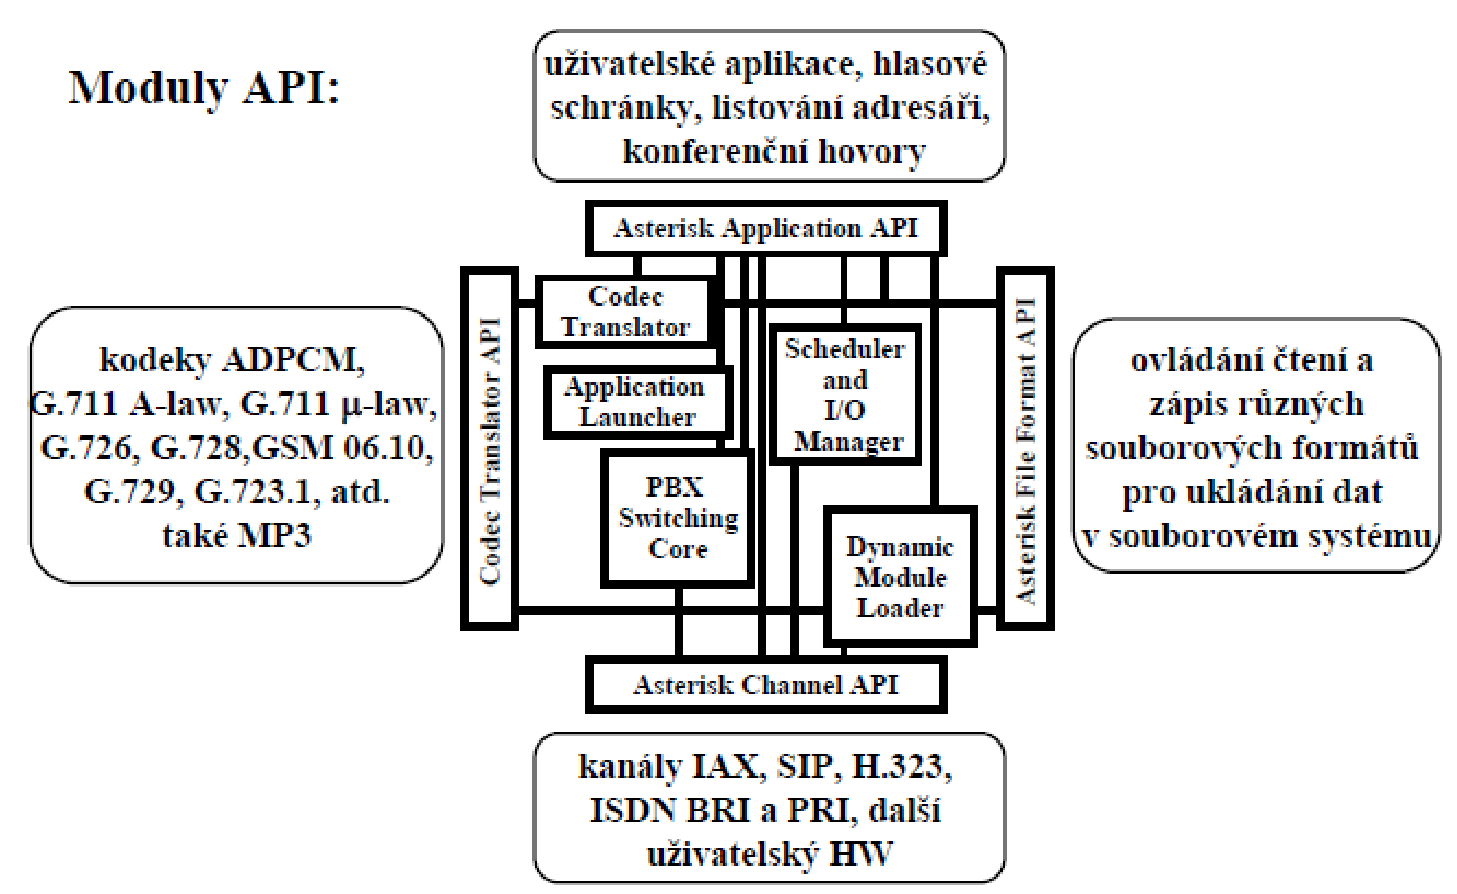
\includegraphics[width=\textwidth]{images/otazka8.png}
        \caption{Architektura PBX Asterisk}
        \label{img:3}
    \end{center}
\end{figure}

\section{Uveďte příklady alternativních Open Source PBX k PBX Asterisk a porovnejte je.}

\begin{figure}[h!]
    \begin{center}
        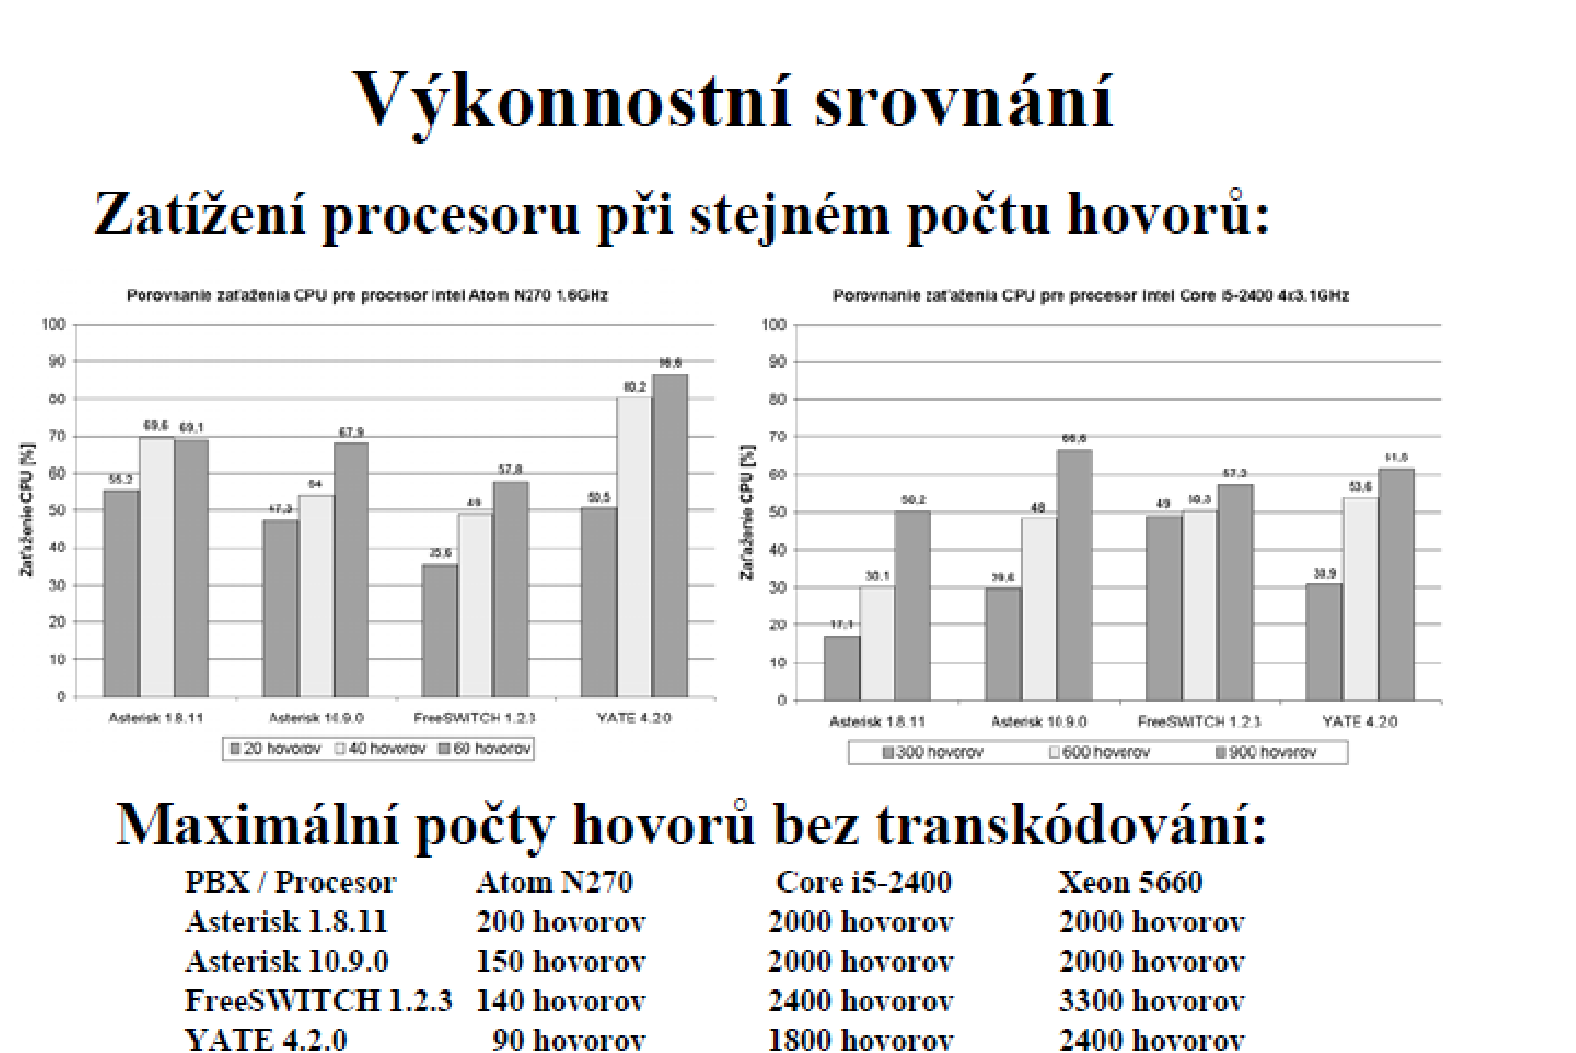
\includegraphics[width=\textwidth]{images/otazka9.png}
        \caption{Alternativní Open Source PBX}
        \label{img:4}
    \end{center}
\end{figure}

\section{Instalace Open Source PBX. Porovnejte výhody a nevýhody instalace z balíčků a instalaci ze zkompilovaných zdrojových souborů. Kdy se pro druhou z nich rozhodnete?}

Instalace z balíčků je jednodužší. Pokud jsem jen uživatel, tak je to jasná volba.
Pokud rozumím UNIX, tak jdu do zkompilovaných zdrojových souborů. Pokud budu chtít modifikovat zdrojové soubory, případně integrovat do Asterisku svůj HW nebo SW.

\section{Uveďte možnosti připojení PBX do veřejné sítě. U jednotlivých příkladů rozhraní uveďte i názvy použitých signalizací.}

\textbf{Embedding} -- jedná se o implementace Softswitchů na jednoúčelových i nepříliš výkonných zařízeních s minimem paměti (např. 4 MB FLASH, 32 MB RAM). Takto lze realizovat například VoIP brány, VoIP ústředny malé Hybridní ústředny. Další možností je implementace přímo na jednoúčelových HW síťových prvcích běžících pod Linuxem. Více informací naleznete např. v Asterisk a embedding.

\textbf{High Availability} (HA) clusters -- zajišťuje pomocí několika počítačů nepřetržité poskytování nějaké služby, v našem případě Softswitche, i při výpadku počítače z důvodu hardwarové závady nebo plánované údržby. Službu poskytuje jeden Softswitch, který je v případě výpadku automaticky zastoupen jiným Softswitchem. Příklad řešení pro Asterisk naleznete v High - Availability Asterisk.

\begin{figure}[h!]
    \begin{center}
        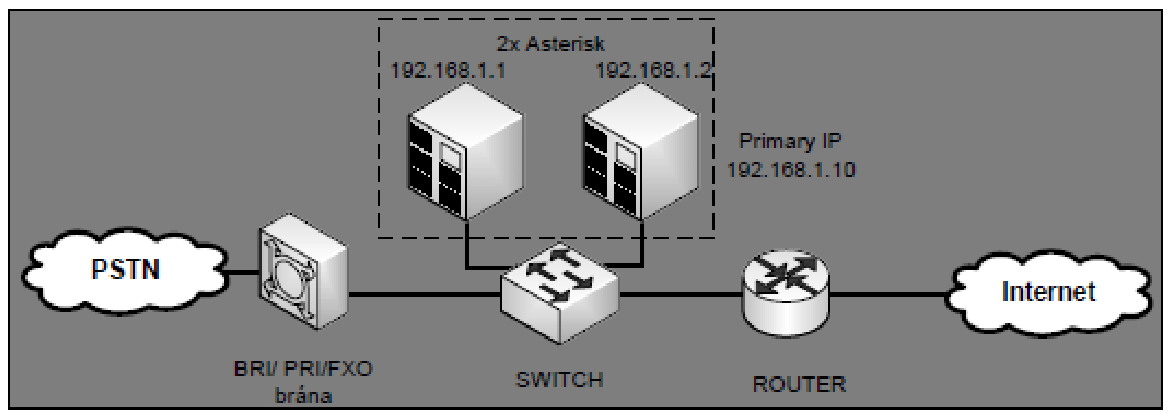
\includegraphics[width=\textwidth]{images/otazka11.png}
        \label{img:5}
    \end{center}
\end{figure}

Rozhraní přenašečů ( trunks ):
umožňující připojení do veřejné sítě a propojení PBX
\begin{itemize}[noitemsep]
    \item Analogové rozhraní označené CO, NDDI (Alcatel), LCOT (Panasonic), TLANI (Siemens), FXO (Asterisk a Open Source), emulující analogový telefon, pouze pro velmi malé ústředny bez IP podpory. - E\&M přenašeč - umožňující realizaci příčky mezi analogovými ústřednami 3. generace, dnes už se nepoužívá.
    \item ISDN T0 - emulující koncové zařízení ISDN BRI 2B+D na sběrnici S0, spíše pro malé ústředny, dnes běžně používáno, ač ISDN pro koncové stanice již nikoli.
    \item E1 přenašeč 2 Mb/s (PCM):
    \begin{itemize}[noitemsep]
        \item E1 s CAS-R2 signalizací (3. generace), dnes už se nepoužívá- ISDN PRI 30B+D (4. generace), běžně používáno.
        \item a další (dnes na Open Source PBX dokonce i se signalizací SS7)
    \end{itemize}
    \item IP trunky se signalizací SIP (H.323, MGCP) nebo proprietárními VoIP signalizačními protokoly. V ústřednách 3. a 4. generace často doplněny VoIP bránou.
    \item GSM brány - pro cenově výhodné volání do GSM sítě nebo v rámci firemní VPN.
\end{itemize}

\section{Vyjmenujte sedm základních funkcí analogové účastnické sady a stručně je vysvětlete. Jak jsou v zahraniční literatuře označeny a-drát a b-drát?}

Každý účastník je zakončen v ústředně na Hlavním Rozvodu (HR) -- Main Distribution Frame (MDF). HR obsahuje i primární přepěťovou ochranu. Odtud je analogový účastník připojen ke své účastnické sadě (ÚSa) pomocí a-drátu (Ring) -Ub a b-drátu (Tip) zem. Parametry tohoto rozhraní definují doporučení ITU-T řady Q.500, ETSI TBR21. Účastnická sada analogové telefonní stanice má tyto funkce:

\begin{itemize}[noitemsep]
    \item Napájení -- Battery
    \item Přepěťové ochrany -- Overvoltage protection
    \item Vyzvánění -- Ringing
    \item Dohlížení -- Supervision
    \item Kódování signálu -- Coding
    \item Vidlicovou funkci -- Hybrid
    \item Testování -- Testing
\end{itemize}

\begin{figure}[h!]
    \begin{center}
        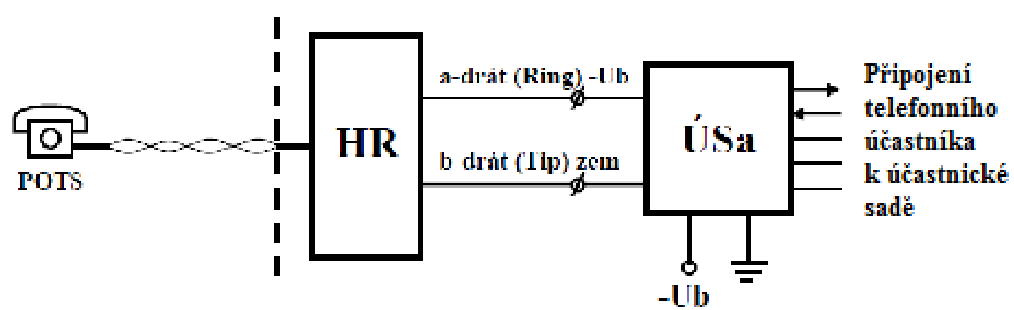
\includegraphics[width=\textwidth]{images/otazka12.png}
        \label{img:6}
    \end{center}
\end{figure}

\section{Funkce účastnické sady: Jakým způsobem je napájen analogový telefon? Specifikujte parametry a typ zdroje.}

\textbf{Napájení} -- Telefonní přístroj je napájen konstantním stejnosměrným proudem většinou cca. 30 mA s napěťovým omezením. Integrované obvody pro účastnické sady umožňují nastavit tento proud v rozsahu cca. 20-60 mA.

V dnešních ústřednách je možno hodnotu proudu nastavit softwarově. V ústřednách prvních generací bylo realizováno napájení z napěťového zdroje přes vinutí relé 2 x 500 . Napájecí napětí zde bylo -60V.

Z historické zvyklosti je uzemněn kladný potenciál (elektrokoroze). Dnes se používá napájecí napětí ve veřejné síti -48 V (prakticky z důvodů nabíjení baterií je kolem -52 V). V pobočkových ústřednách je napětí nižší, zpravidla 24 V.

Napájení konstantním zdrojem proudu umožňuje minimalizovat vliv délky vedení na napájení telefonního přístroje. Mezní parametry vedení jsou 2 x 800 a 0,5 $\mu$F (vedení 0,4mm ~ 270 /km, Rtelefonu = 600 ).

\section{Funkce účastnické sady: Vysvětlete funkce analogové účastnické sady vyzvánění, dohlížení a testování. Dle specifické funkce uveďte parametry úrovní a tvaru signálů, časové parametry.}

\textbf{Vyzváněné (Ringing)}

Vyzvánění je realizováno střídavým napětím o efektivní hodnotě 75 V, 25±2 Hz superponovaným na záporné napětí baterie -Ub. Vyzvánění je přerušovaný signál zvonění/mezera 1/4 s. U pobočkových ústředen se používají i jiné kombinace (např. 0,3/0,3/0,3/4 s) pro zvonění z vnitřní linky PBX.

V moderních PBX lze definovat vlastní. Telefon by měl být schopen detekovat už 25 V efektivních. V mezeře mezi prvním a druhým zvoněním se přenáší CLIP (identifikace volajícího).

\noindent\textbf{Dohlížení (Supervision)}

Jedná se o dohled nad stavem účastníka (vyvěšeno/zavěšeno). V podstatě účastnická sada sleduje stejnosměrný proud smyčky a předává tuto informaci dále. Stejnosměrný proud smyčky při zavěšení musí být menší než 0,5 mA (typicky 0,05mA), detekuje se pokles o 2 mA, odpor smyčky je větší než 100 k (typicky větší než 1 M).

Stejnosměrný proud smyčky při vyvěšení je 15 až 60 mA, odpor smyčky je menší než 2 k. Na základě doby trvání a logickém stavu je vyhodnoceno zdali se jedná o vyzvednutí (uzavření proudové smyčky po dobu delší než 300ms), zavěšení (přerušení proudu smyčky na dobu delší než 400ms), pulsní volbu (pulsy 40/60ms) či signál FLASH (30-180 ms).

\noindent\textbf{Testování (Testing)}

Testovací obvody obsahují PSTN ústředny, ale PBX zpravidla ne. IO pro účastnické sady testovací obvody většinou neobsahují. Účastnická sada obsahuje několik relé T a S, které přivedou části testované účastnické sady a účastnického vedení do testovací jednotky (zpravidla jiná sdílená karta).

Testuje se impedance vedení, svod vedení, ochranné obvody pomocí definovaných impulsů, počet připojených přístrojů, měření při zavěšení i vyvěšení, účastníka je možno odvést do speciální měřicí ÚSa, automatické testování v noci.

\section{Funkce účastnické sady: Vysvětlete funkce analogové účastnické sady kódování a vidlicovou funkci. Pro které generace ústředen jsou tyto funkce vyžadovány?}

\textbf{Coding} -- Vdigitálních ústřednách je potřeba realizovat digitalizaci analogového signálu. Analogový signál je nutno kmitočtově omezit na 0,3-3,4 kHz (dnešní ústředny i o trošku více), navzorkovat \uv{8 kHz} (dnes předvzorkováno vyšším kmitočtem, což umožňuje jednodušší číslicovou filtraci a další číslicové zpracování), realizovat datovou kompresi (A-law) a vytvořit tak výsledný datový tok 64 kb/s. IO pro tyto účely obsahuje tedy kodér, dekodér a filtry, a proto se označuje COFIDEC.

\noindent\textbf{Coding} -- Tyto integrované obvody umožňují programovatelně nastavit zesílení, vstupní impedanci, vyvážení vidlice a vlastní přenosovou funkci filtrů. Součástí těchto obvodů je i číslicový tónový generátor umožňující generovat tónovou výbavu, vyzváněcí signál a signál pro identifikaci volajícího (CLIP).

\noindent\textbf{Hybrid} -- Vidlice zajišťuje převod 2-drátu na 4-drát, což je nezbytná operace pro následnou digitalizaci signálu. Dnes je řešena jako aktivní pomocí operačních zesilovačů. Softwarově lze nastavit jestli je účastník připojen krátkým, středně dlouhým nebo dlouhým vedením. Většinou však je nastaveno jednotně pro celou ústřednu. Vzniklé echo od nedokonalého vyvážení je minimalizováno při následném číslicovém zpracování signálu.

\section{Vysvětlete signalizaci na analogovém účastnickém rozhraní POTS pro stav \uv{volání}. Uveďte reprezentaci jednotlivých signálů a jejich parametry. Jedná se o celosvětově standardní signalizaci nebo se v jednotlivých zemích liší?}

Signalizace U na analogovém účastnickém rozhraní:
\begin{itemize}[noitemsep]
    \item Jedná se o přístupovou obousměrnou asymetrickou signalizaci využívanou při komunikaci s běžným analogovým telefonem (POTS).
\end{itemize}

\noindent Signalizace pro stav \uv{VOLÁNÍ}:
\begin{figure}[h!]
    \begin{center}
        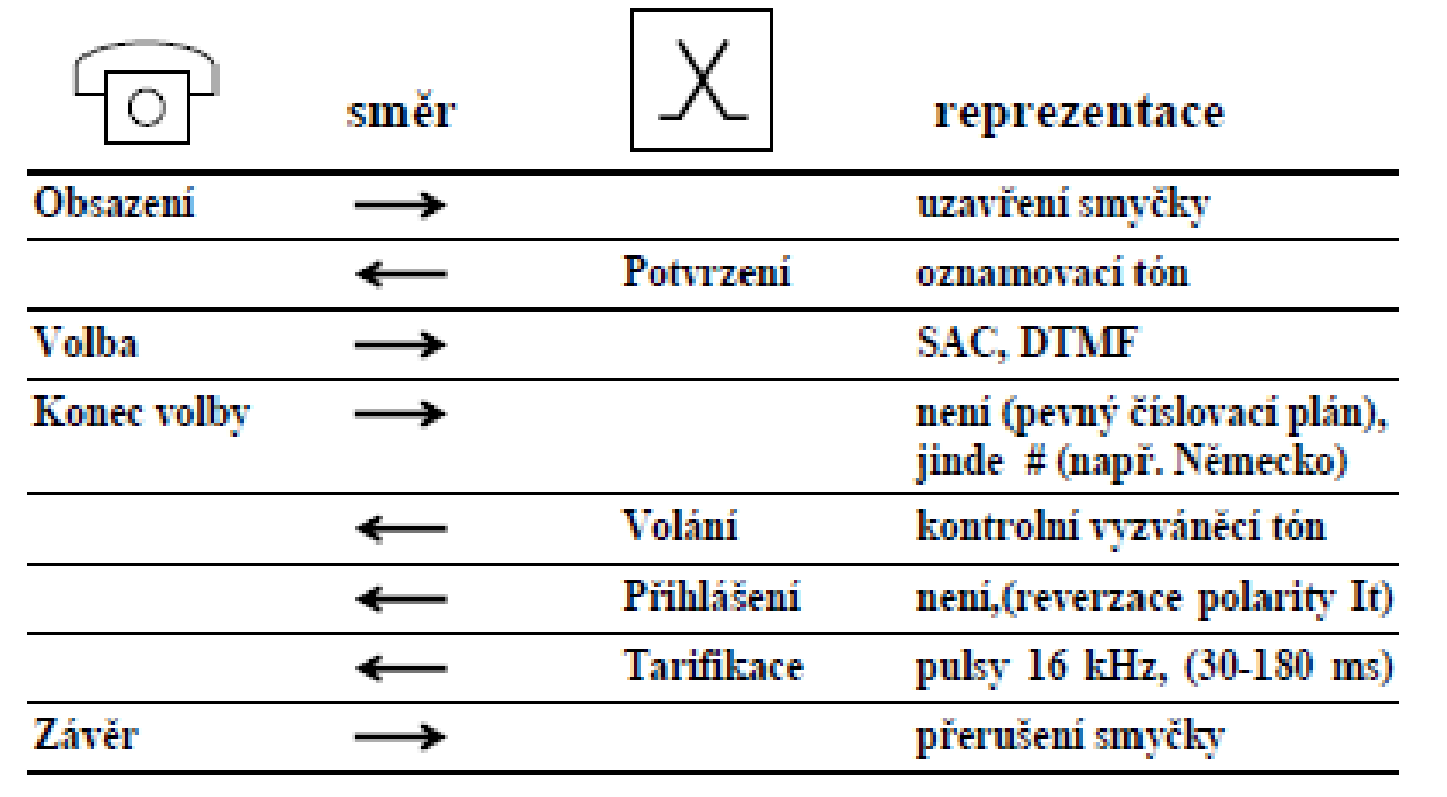
\includegraphics[width=\textwidth]{images/otazka16.png}
        \label{img:7}
    \end{center}
\end{figure}

\noindent Signalizace U se v jednotlivých zemích liší!

\noindent Příklady:
\begin{itemize}[noitemsep]
    \item V ČR neexistuje reprezentace pro přihlášení volaného, zatímco v Itálii dochází k reverzaci polarity napájení telefonního přístroje.
    \item V ČR se nepoužívá reprezentace ukončení volby, protože používáme pevný číslovací plán (pevná délka telefonního čísla).
    \item V Německu a v řadě jiných zemí není pevný číslovací plán a je potřeba zakončit volbu znakem \#. Toto zakončení je potřeba i u nás při volání do zahraničí. Jinak je nutno čekat 8 sekund, po kterých považuje ústředna volbu za kompletní.
    \item V UK společnost British Telecom používá ještě před prvním vyzváněním reverzaci polarity, a poté ještě před prvním zazvoněním je přenesena identifikace volajícího CLIP.
\end{itemize}

\section{Jaké hardwarové karty pro Open Source PBX jsou dnes nabízeny?}

Hardware pro Softswitche: Výrobci HW jsou Digium, Sangoma, BeroNet a další. Firma Digium je hlavním sponzorem projektu Asterisk.

Analogove karty, Karty ISDN BRI 2B+D, Karty E1 ISDN -- PRI 30B+Dm, Modul potlačenia ozveny, Transkodovacie karty, GSM karty.

FXS (Foreign eXchange Subscriber) zásuvka na zdi, přináší telefonní služby od telefonní společnosti směrem k uživateli (vyzváněcí tón, vyzváněcí napětí, apod.)

FXO ( Foreign eXchange Office) zásuvka na telefonu, zajišťuje směr zákazník -- telefonní společnost. (zdroj signálu pro přihlášení a odhlášení)

\section{Jaké jsou základní prvky signalizační sítě SS7? Vysvětlete jejich funkci.}

Základní prvky signalizační sítě SS7 jsou signalizační body SP (Signal Point):

SSP (Service Switching Point) -- koncový bod signalizace, který generuje signalizaci a zpracovává signalizaci. Je to vlastně telefonní ústředna. Mezi SSP je možno přenášet jak signalizaci SS7, tak hovorová data.

STP (Signal Transfer Point) -- nezpracovává signalizaci, pouze ji předává. Je obdobou switche v IP sítích. SCP (Service Control Point) -- stejně jako SSP je koncovým bodem signalizace a generuje i zpracovává signalizaci. Obsahuje databázi všech SP.

\begin{figure}[h!]
    \begin{center}
        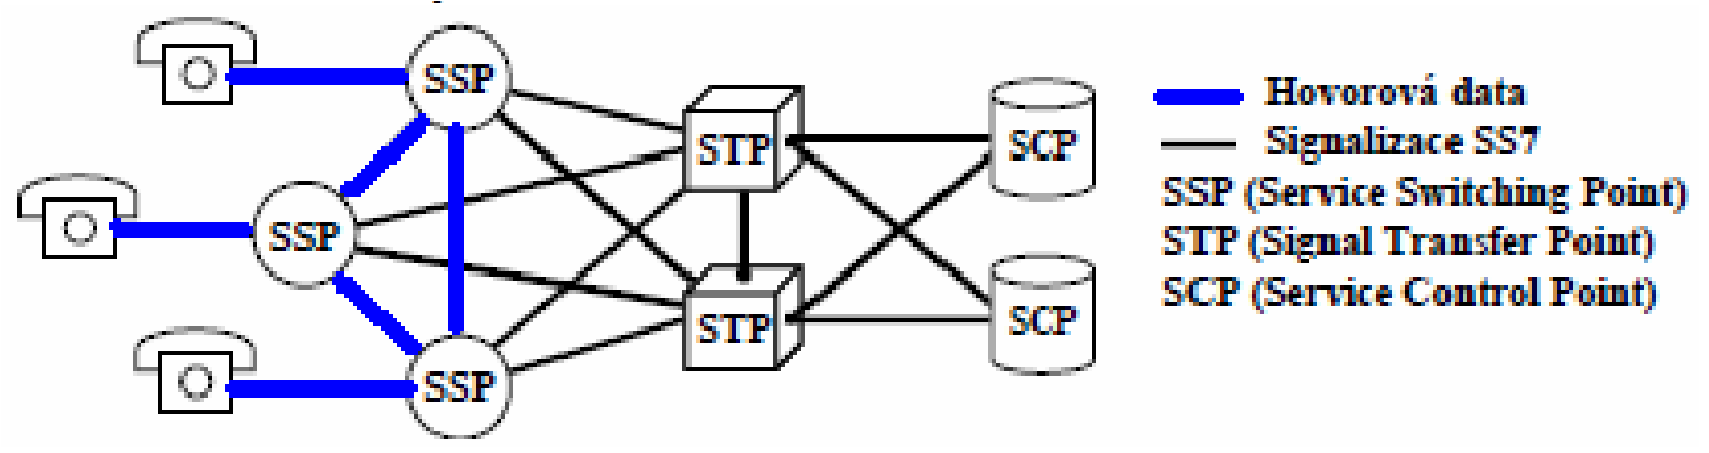
\includegraphics[width=\textwidth]{images/otazka18.png}
        \label{img:8}
    \end{center}
\end{figure}

\section{Jakým způsobem je řešena adresace v síti SS7. Vysvětlete význam pojmu národní síť, národní rezerva (přechodová síť), mezinárodní síť, mezinárodní rezerva? Zakreslete obrázek využití jednotlivých sítí v ČR.}

Struktura sítě SS7 je tvořena body SP (Signaling Point). Každý signalizační bod má svojí adresu, která se nazývá SPC (Signaling Point Code) a má délku 14 bitů. Zóna (první 3 bity) odpovídá přibližně světadílu, dále je specifikována zem (identifikace sítě 8 bitů) v rámci zóny a pak následuje vlastní identifikace (adresa) SP (3 bity). Adresa SP je rozdělena do tří úrovní: mezinárodní, národní (mezi-operátorová) a operátorová. Důvod tohoto dělení spočívá ve zjednodušení přidělování SPC.

Mezinárodní SPC přiděluje ITU a na národní úrovni se o přidělování stará telekomunikační úřad, v našem případě ČTÚ. Ke kódu SPC se přidává identifikátoru NI (Network Indicator -- 2 bity), který slouží pro přenos mezi sítěmi SS7.

Ten specifikuje zdali se jedná o SPC v národní síti NAT0-národní síť a NAT1-národní rezerva nebo INAT0-mezinárodní síť a INAT1-mezinárodní rezerva. NAT0 je síť operátora, NAT1 je síť propojující operátory v rámci dané země. INAT 0 je mezinárodní síť SS7, ve které jsou umístěny mezinárodní ústředny jednotlivých operátorů. INAT1 umožňuje vytvořit síť nad sítěmi mezinárodních INAT0.

\begin{figure}[h!]
    \begin{center}
        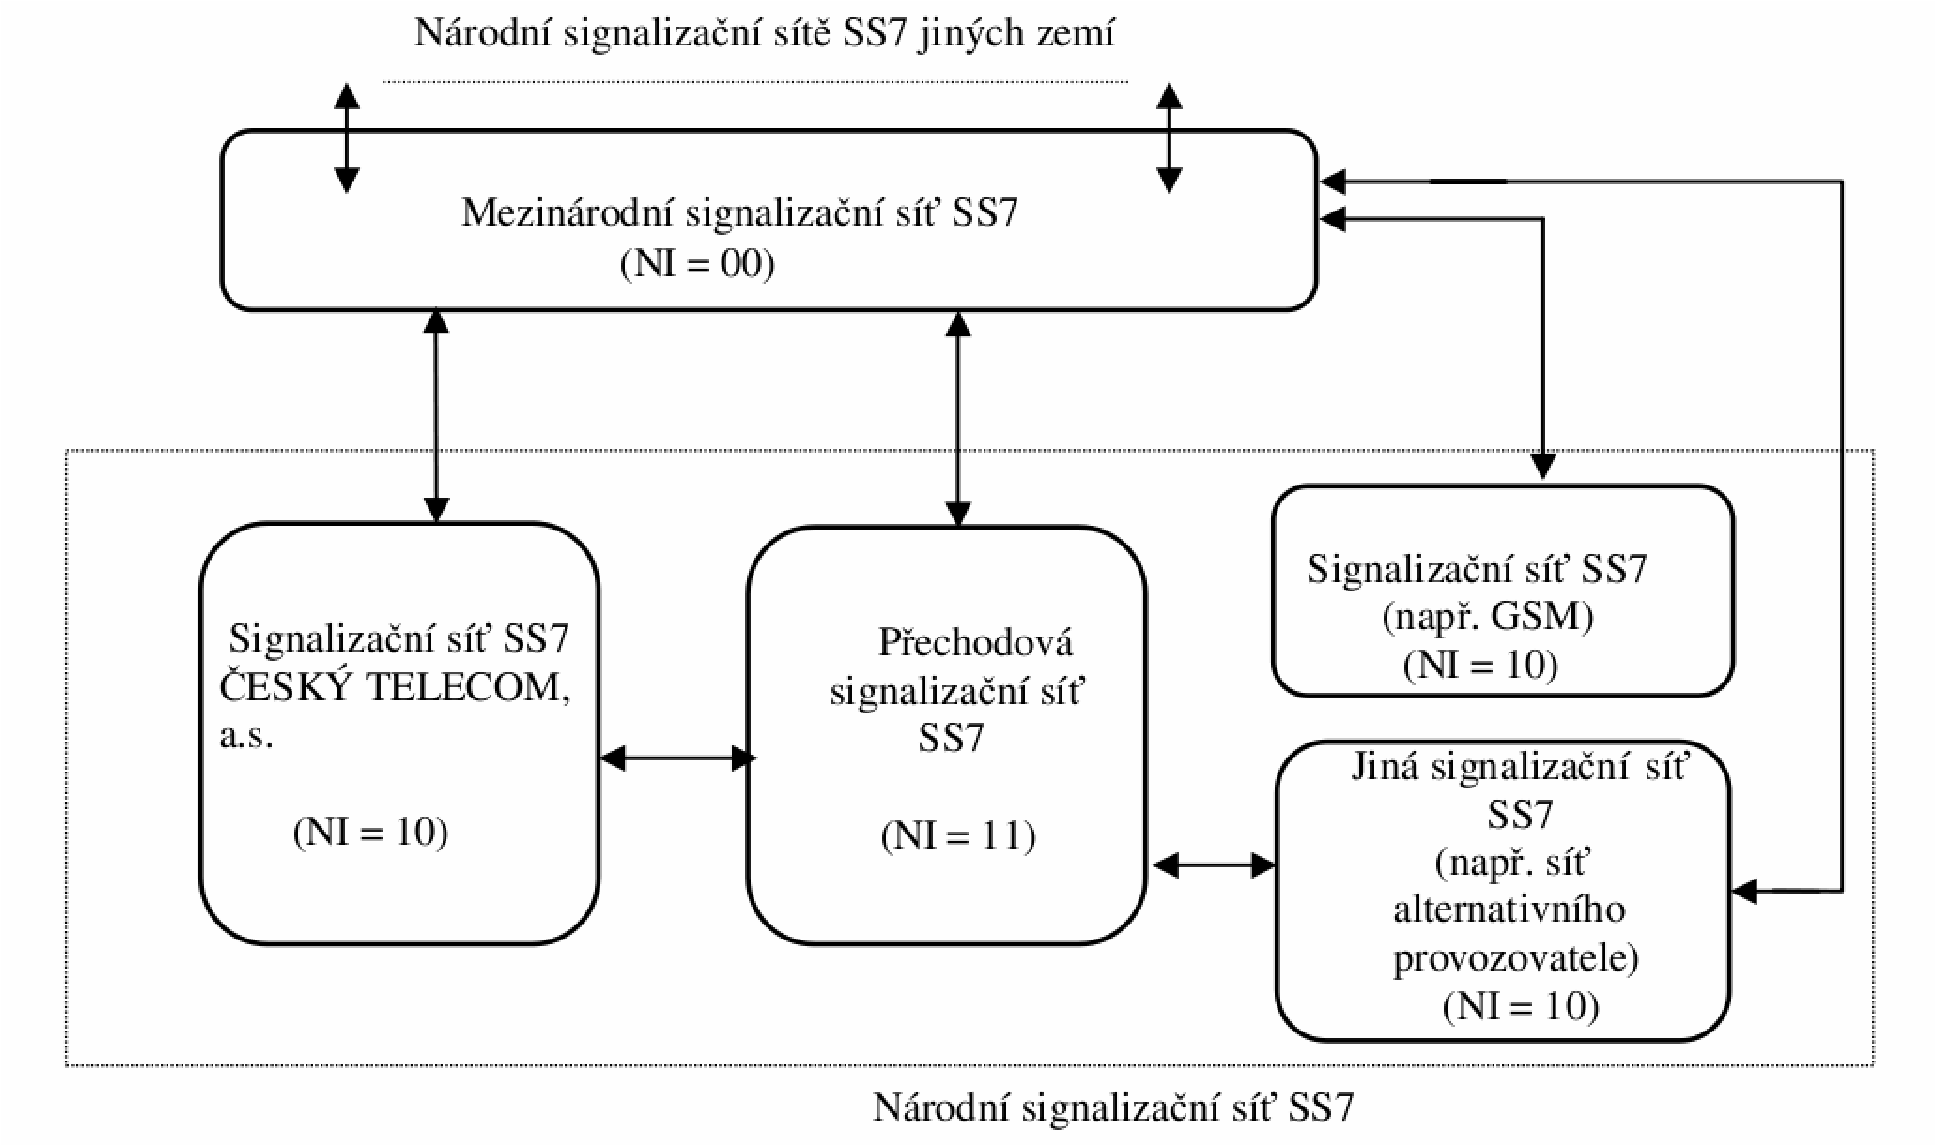
\includegraphics[width=\textwidth]{images/otazka19.png}
        \label{img:9}
    \end{center}
\end{figure}

\section{SS7: Uveďte základní tři typy zpráv (SU) přenášených na 2. vrstvě. K čemu slouží?}

FISU -- (Fill-in Signal Units) jsou tzv. výplňové zprávy. Jsou vysílány neustále a zajišťují pravidelnou bitovou strukturu. Dále slouží k potvrzování zpráv MSU.

LSSU - (Link Status Signal Units) používající se k indikaci stavu signalizačních bodů (SP)/linky a tzv. zarovnání (alignment). Přenáší tyto stavy linky: SIO (Out of Alignment) normální/rychlé zarovnání, SIN/SIE (Normal/EmergencyAlignment). SIOS -- SP mimo provoz, SIPO -- SP je nedostupný pro vyšší protokoly, SIB -- zahlceni SP

MSU - (Message Signal Units) zprávy, které přenáší užitečnou informaci. Obsahuje: SIO (Service Information Octet) -- typ sítě (národní/mezinárodní), prioritu a typ zprávy. SIF (Signaling Information Field) -- zdroj, cíl, cestu zprávy a signalizační informace.

\section{SS7: Jakým způsobem je identifikováno v signalizací SS7-ISUP, která může probíhat i v zcela jiném rámci E1 než vlastní hovor, ke kterému time-slotu a E1 tato signalizace přísluší.}

CIC (Circuit Identification Code) udává okruh pro který se buduje hovor.

Pokud je signalizační linka i hovorový okruh v téže E1, je vyšší část CIC nulová a v nižší je přímo číslo kanálu. Druhou variantou je sloučení více skupin E1, pak vyšší část CIC určuje skupinu, tedy o kterou E1 jde. Nižší opět určuje kanál. DODATEK - Jedná se o informaci 3.vrstvy pro vrstvu ISUP.

\section{SS7: Uveďte sled zprávy, které se přenáší na vrstvě ISUP při budování hovorového spojení.}

- vrstva ISUP = ISDN user part

\begin{figure}[h!]
    \begin{center}
        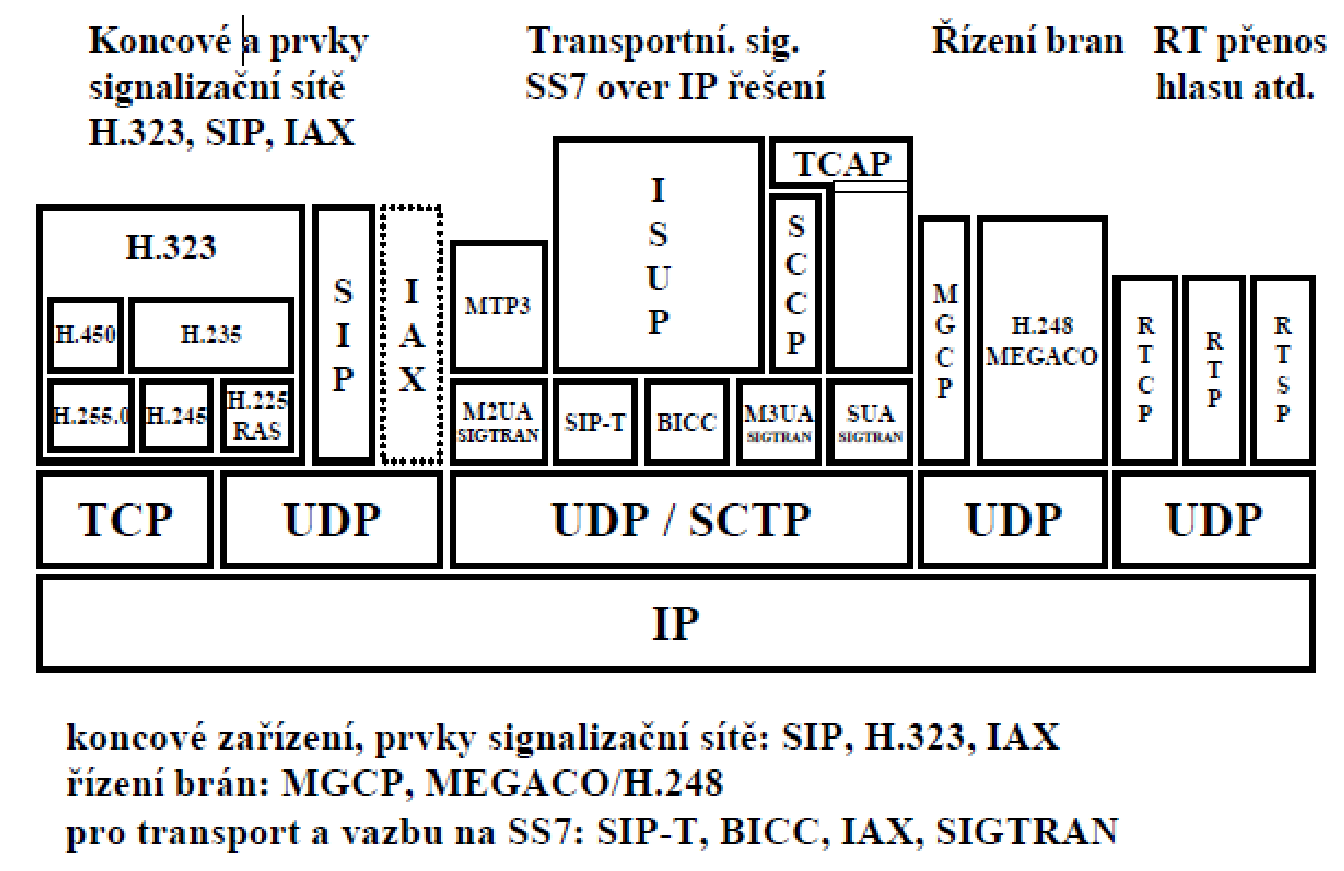
\includegraphics[width=\textwidth]{images/otazka25.png}
        \label{img:10}
    \end{center}
\end{figure}

\begin{itemize}[noitemsep]
    \item IAM (Initial Address) -- žádost o spojení a adresní informace
    \item ACM (Address Complete) -- kladná odpověď na žádost o spojení
    \item ANM (Answer) -- volaný účastník vyzvednul
    \item REL (Release) -- zrušit hovor
    \item RLC (Release Complete) -- potvrzení zrušení
\end{itemize}

\section{SS7: Uveďte, ve kterých Open Source PBX a jak lze implementovat SS7. Rovněž u každého příkladu uveďte, které prvky signalizační sítě SS7 jsou implementovány.}

Implementace signalizačního systému číslo 7 pro Asterisk na bázi TDM:
\begin{itemize}[noitemsep]
    \item Chan SS7 - channel driver pro implementaci SS7 na rozhranní E1 a hardware kompatibilním s produkty firmy Digium. Chan\_ss7 byl vyvinut společností SIFIRA, avšak zdrojový kód byl uvolněn. Kompatibilní s Asteriskem verze 1.4, 1.6 a 1.8. V Asterisku je doplněn další kanál chan\_ss7.
\end{itemize}

Další informace na \href{http://www.netfors.com/chan_ss7_free}{http://www.netfors.com/chan\_ss7\_free}.

\begin{itemize}[noitemsep]
    \item LibSS7 - pochází podobně jako LibPri (ISDN PRI) přímo od vývojářů Asterisku, firmy Digium. Jedná se opět o rozšíření chan\_dahdi. Popis instalace a konfigurace viz dále.
    \item SS7box / SS7boost - placené řešení firmy Sangoma. Skládá se z prvků Sangoma Media Gateway, SS7box, SS7boost. Na Asterisk je navázána pomocí chan\_woomera (viz Sangoma BRI). Umožňuje i přenos SS7 signalizace přes IP síť protokolem SCTP viz dále.
\end{itemize}

\section{Uveďte standardizované signalizační VoIP protokoly a oblast využití.}

Nejznámějšími signalizačními protokoly v internetové telefonii VoIP jsou:
\begin{itemize}[noitemsep]
    \item SIP (Session Initiation Protocol - IETF)
    \item skupina protokolů H.323 (ITU-T)
    \item MGCP (Media Gateway Control Protocol - IETF, ITU-T)
    \item H.248/MEGACO (ITU-T)
    \item v poslední době i protokol tvůrců PBX Asterisk IAX (Inter - Asterisk eXchange -- IETF)
\end{itemize}
Dle kategorizace z předchozí hodiny lze označit SIP, H.323 a v poslední době i IAX jako přístupové signalizační protokoly. Protokol H.323 je už pro koncové VoIP zařízení na ústupu. MGCP, MEGACO a H.248 jsou protokoly řízení bran.

Proprietární signalizační protokoly, zejména v PBX:
\begin{itemize}[noitemsep]
    \item NOE (New Office Environment) -- Alcatel-Lucent
    \item SCCP (Skinny Client Control Protocol) -- CISCO
    \item PTAP (Panasonic Telephony Administration Protocol) -- Panasonic
    \item CorNet-IP (Corporate) - HFA (HiPath Feature Access), -- Siemens
    \item Skype
\end{itemize}

\section{K čemu slouží protokoly pro správu multimediální relace, co je v nich přenášeno, co je pomocí nich \uv{vyjednáváno}. Uveďte protokoly pro správu multimediální relace využívané v SIP, MGCP, H.323 a IAX.}

Signalizační protokoly pro vazbu na signalizační systém SS7 a jeho přenos po IP síti:
\begin{itemize}[noitemsep]
    \item SIP-T (Session Initiation Protocol for Telephones -- IETF),- BICC (Bearer Independent Call Control -- ITU-T), - SIGTRAN (SIGnaling TRANslation - IETF).
\end{itemize}

Protokoly pro správu multimediální relace:
\begin{itemize}[noitemsep]
    \item SDP (Session Description Protocol - IETF) - v SIP, MGCP, \ldots
    \item H.245 (ITU-T) - v H.323, H.248/MEGACO, \ldots
\end{itemize}

Protokoly pro real-time multimediální přenos:
\begin{itemize}[noitemsep]
    \item RTP (Real-time Transport Protocol - IETF) - SRTP (Secure Real-time Transport Protocol - IETF)
\end{itemize}

Standardy kodeků:
\begin{itemize}[noitemsep]
    \item ITU.T řady G: G.711, G.729, G.723.1, G.726, \ldots ( řada H - video) - ostatní: GSM, iLBC, AMR, Speex, \ldots
\end{itemize}

\section{Protokol SIP: Popište průběh spojení. Co zajišťuje SDP protokol a kde se přenáší. Jaký je jeho ekvivalent v H.323 protokolu.}

Protokol SIP (Session Initiation Protocol): signalizační textový protokol,komunikace bod-bod

Zajišťuje:
\begin{itemize}[noitemsep]
    \item sestavení spojení mezi 2 či více účastníky
    \item dohled(modifikaci) na používáním tohoto spojení
    \item rušení spojení
    \item sestavení spojení mezi 2 či více účastníky
    \item sestavení spojení mezi 2 či více účastníky
\end{itemize}
NEŘEŠÍ: řízení hovoru, tj. dohadování parametrů na schopnostech zařízení -- použitých kodecích atd.

Průběh spojení:
\begin{figure}[h!]
    \begin{center}
        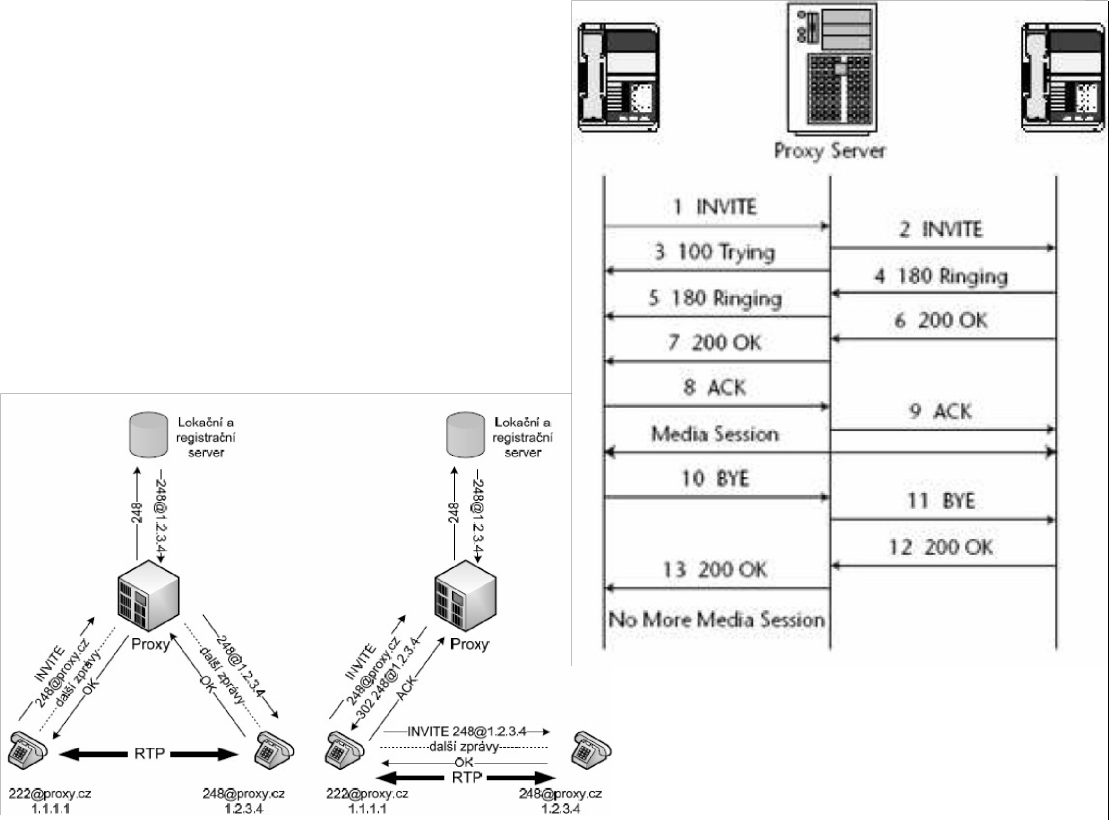
\includegraphics[width=\textwidth]{images/otazka26.png}
        \caption{Srovnání - Open source vs. Proprietary}
        \label{img:11}
    \end{center}
\end{figure}

Co zajišťuje SDP a kde se přenáší

SDP (Session Description Protocol) zajišťuje vyjednání parametrů spojení např:
\begin{itemize}[noitemsep]
    \item kodeky
    \item metody šifrování
    \item rušení spojení
    \item vyžadovaná šírka pásma
\end{itemize}

SDP je umístěn v požadavcích/odpovědích SIP, jestliže je umístěno -- Contend-type:application/SDP, pak data požadavku/odpovědi SIP obsahují SDP.

Jaký je ekvivalent v H.323 protokolu

SIP -- H.225

SDP -- H.245

\section{Protokol SIP: Vysvětlete odlišnosti v implementaci SIP proxy a B2BUA (Back to Back User Agent). Zakreslete obrázky. Která z uvedených metod je uplatněna v PBX Asterisk a jaké jsou její výhody?}

B2BUA plní funkci proxy serveru a zároveň představuje koncový bod pro signalizaci. Na rozdíl od proxy může vytvářet spojení a zasahovat do zasílaných zpráv a při komunikaci mezi koncovými účastníky. SIP proxy architektura je rychlejší, než B2BUA, protože se zabývá pouze signalizacemi. B2BUA může být velmi pomalá díky tomu, že je využita jako SIP proxy pro překlad kodeků z jednoho na druhý (např. G.729 <-> G.711, překlad SIP na H.323). V Asterisku je uplatněna B2BUA.

\section{Vysvětlete rozdíl účtů user, peer a friend v PBX Asterisk. Zakreslete model autentizace hovoru v PBX Asterisk.}

Lorem ipsum dolor sit amet, consectetur adipiscing elit. Nullam vehicula vestibulum felis, hendrerit aliquet sapien sodales nec. Phasellus semper quis orci at ultricies. Mauris non magna vitae massa faucibus vestibulum vel id lorem. Vestibulum interdum lobortis nisl, ut rhoncus dui facilisis sed. Donec eget accumsan lectus. Etiam metus leo, tempus vitae velit non, sagittis tempus dui. Vestibulum nec consectetur velit.

\section{Protokol IAX: Popište protokol IAX. Uveďte dva typy rámců, a kdy se který z nich využívá. Popište odlišnosti oproti protokolům SIP a H.323. Uveďte sled zpráv přenášených při budování spojení.}

Lorem ipsum dolor sit amet, consectetur adipiscing elit. Nullam vehicula vestibulum felis, hendrerit aliquet sapien sodales nec. Phasellus semper quis orci at ultricies. Mauris non magna vitae massa faucibus vestibulum vel id lorem. Vestibulum interdum lobortis nisl, ut rhoncus dui facilisis sed. Donec eget accumsan lectus. Etiam metus leo, tempus vitae velit non, sagittis tempus dui. Vestibulum nec consectetur velit.

\section{Popište signalizační protokol MGCP. Uveďte oblast jeho využití. Uveďte zprávy (příkazy) používané při vytváření spojení.}

Lorem ipsum dolor sit amet, consectetur adipiscing elit. Nullam vehicula vestibulum felis, hendrerit aliquet sapien sodales nec. Phasellus semper quis orci at ultricies. Mauris non magna vitae massa faucibus vestibulum vel id lorem. Vestibulum interdum lobortis nisl, ut rhoncus dui facilisis sed. Donec eget accumsan lectus. Etiam metus leo, tempus vitae velit non, sagittis tempus dui. Vestibulum nec consectetur velit.

\section{Uveďte alespoň některé proprietární signalizační VoIP protokoly a oblast využití.}

Lorem ipsum dolor sit amet, consectetur adipiscing elit. Nullam vehicula vestibulum felis, hendrerit aliquet sapien sodales nec. Phasellus semper quis orci at ultricies. Mauris non magna vitae massa faucibus vestibulum vel id lorem. Vestibulum interdum lobortis nisl, ut rhoncus dui facilisis sed. Donec eget accumsan lectus. Etiam metus leo, tempus vitae velit non, sagittis tempus dui. Vestibulum nec consectetur velit.

\section{K čemu slouží skupina protokolů SIGTRAN? Nakreslete vazbu TDM a IP sítě s využitím protokolu SIGRAN.}

Lorem ipsum dolor sit amet, consectetur adipiscing elit. Nullam vehicula vestibulum felis, hendrerit aliquet sapien sodales nec. Phasellus semper quis orci at ultricies. Mauris non magna vitae massa faucibus vestibulum vel id lorem. Vestibulum interdum lobortis nisl, ut rhoncus dui facilisis sed. Donec eget accumsan lectus. Etiam metus leo, tempus vitae velit non, sagittis tempus dui. Vestibulum nec consectetur velit.

\section{Jaké jsou možnosti přenosu DTMF tónů ve VoIP telefonii. Uveďte příklady aplikací, kdy je nutno přenášet DTMF?}

Lorem ipsum dolor sit amet, consectetur adipiscing elit. Nullam vehicula vestibulum felis, hendrerit aliquet sapien sodales nec. Phasellus semper quis orci at ultricies. Mauris non magna vitae massa faucibus vestibulum vel id lorem. Vestibulum interdum lobortis nisl, ut rhoncus dui facilisis sed. Donec eget accumsan lectus. Etiam metus leo, tempus vitae velit non, sagittis tempus dui. Vestibulum nec consectetur velit.

\section{Co je to NAT? Vysvětlete problematiku NAT a problematiku SIP klienta v podsíti. Vysvětlete funkci protokolu STUN. Pro který typ NATu jej nelze použít a proč? Jaké znáte další možnosti \uv{překonání} NAT? Jak je řešen tento problém v PBX Asterisk?}

Lorem ipsum dolor sit amet, consectetur adipiscing elit. Nullam vehicula vestibulum felis, hendrerit aliquet sapien sodales nec. Phasellus semper quis orci at ultricies. Mauris non magna vitae massa faucibus vestibulum vel id lorem. Vestibulum interdum lobortis nisl, ut rhoncus dui facilisis sed. Donec eget accumsan lectus. Etiam metus leo, tempus vitae velit non, sagittis tempus dui. Vestibulum nec consectetur velit.

\section{QoS ve VoIP: Jaké jsou základní tři metody hodnocení kvality hovoru? Co je to MOS a jakých hodnot může nabývat? Co je to R-faktor? Uveďte i některé konkrétní metody.}

Lorem ipsum dolor sit amet, consectetur adipiscing elit. Nullam vehicula vestibulum felis, hendrerit aliquet sapien sodales nec. Phasellus semper quis orci at ultricies. Mauris non magna vitae massa faucibus vestibulum vel id lorem. Vestibulum interdum lobortis nisl, ut rhoncus dui facilisis sed. Donec eget accumsan lectus. Etiam metus leo, tempus vitae velit non, sagittis tempus dui. Vestibulum nec consectetur velit.

\section{Uveďte některé zvukové kodeky. Je použití některých kodeků licencováno? Uveďte některé z nich. Které kodeky jsou standardně implementovány v HW koncových zařízeních a PBX tradičních výrobců.}

Lorem ipsum dolor sit amet, consectetur adipiscing elit. Nullam vehicula vestibulum felis, hendrerit aliquet sapien sodales nec. Phasellus semper quis orci at ultricies. Mauris non magna vitae massa faucibus vestibulum vel id lorem. Vestibulum interdum lobortis nisl, ut rhoncus dui facilisis sed. Donec eget accumsan lectus. Etiam metus leo, tempus vitae velit non, sagittis tempus dui. Vestibulum nec consectetur velit.

\section{QoS ve VoIP: Jak souvisí zpoždění paketů s ozvěnou (echem)? Jaké zpoždění signálu bylo v TDM sítích a jaké je cca. v paketových sítích?}

Lorem ipsum dolor sit amet, consectetur adipiscing elit. Nullam vehicula vestibulum felis, hendrerit aliquet sapien sodales nec. Phasellus semper quis orci at ultricies. Mauris non magna vitae massa faucibus vestibulum vel id lorem. Vestibulum interdum lobortis nisl, ut rhoncus dui facilisis sed. Donec eget accumsan lectus. Etiam metus leo, tempus vitae velit non, sagittis tempus dui. Vestibulum nec consectetur velit.

\section{QoS ve VoIP: Jakými způsoby je možno zajistit QoS ve VoIP telefonii? Je podpora některé z metod zajištění QoS ve VoIP zařízeních téměř standardně implementována? Vysvětlete pojmy DSCP, třída EF (Expedited Forwarding), VoIP VLAN (IEEE 802.1p).}

Lorem ipsum dolor sit amet, consectetur adipiscing elit. Nullam vehicula vestibulum felis, hendrerit aliquet sapien sodales nec. Phasellus semper quis orci at ultricies. Mauris non magna vitae massa faucibus vestibulum vel id lorem. Vestibulum interdum lobortis nisl, ut rhoncus dui facilisis sed. Donec eget accumsan lectus. Etiam metus leo, tempus vitae velit non, sagittis tempus dui. Vestibulum nec consectetur velit.

\section{Bezpečnost IP telefonie: Jaké znáte typy útoků na telefonní provoz v IP síti. Uveďte alespoň některá opatření k zajištění bezpečnosti VoIP telefonie.}

Lorem ipsum dolor sit amet, consectetur adipiscing elit. Nullam vehicula vestibulum felis, hendrerit aliquet sapien sodales nec. Phasellus semper quis orci at ultricies. Mauris non magna vitae massa faucibus vestibulum vel id lorem. Vestibulum interdum lobortis nisl, ut rhoncus dui facilisis sed. Donec eget accumsan lectus. Etiam metus leo, tempus vitae velit non, sagittis tempus dui. Vestibulum nec consectetur velit.

\section{Bezpečnost IP telefonie: Jaké znáte možnosti a protokoly realizace šifrovaného přenosu VoIP telefonie (signalizace i \uv{hlasu})? Uveďte důvody, proč se zatím v širší míře neuplatňují.}

Lorem ipsum dolor sit amet, consectetur adipiscing elit. Nullam vehicula vestibulum felis, hendrerit aliquet sapien sodales nec. Phasellus semper quis orci at ultricies. Mauris non magna vitae massa faucibus vestibulum vel id lorem. Vestibulum interdum lobortis nisl, ut rhoncus dui facilisis sed. Donec eget accumsan lectus. Etiam metus leo, tempus vitae velit non, sagittis tempus dui. Vestibulum nec consectetur velit.

\section{Vysvětlete pojmy zjevný, skrytý, otevřený a uzavřený číslovací plán.}

Lorem ipsum dolor sit amet, consectetur adipiscing elit. Nullam vehicula vestibulum felis, hendrerit aliquet sapien sodales nec. Phasellus semper quis orci at ultricies. Mauris non magna vitae massa faucibus vestibulum vel id lorem. Vestibulum interdum lobortis nisl, ut rhoncus dui facilisis sed. Donec eget accumsan lectus. Etiam metus leo, tempus vitae velit non, sagittis tempus dui. Vestibulum nec consectetur velit.

\section{Vysvětlete pojem omezení oprávnění v PBX. Jak je implementováno v tradičních PBX a jak je lze implementovat v PBX Asterisk.}

Lorem ipsum dolor sit amet, consectetur adipiscing elit. Nullam vehicula vestibulum felis, hendrerit aliquet sapien sodales nec. Phasellus semper quis orci at ultricies. Mauris non magna vitae massa faucibus vestibulum vel id lorem. Vestibulum interdum lobortis nisl, ut rhoncus dui facilisis sed. Donec eget accumsan lectus. Etiam metus leo, tempus vitae velit non, sagittis tempus dui. Vestibulum nec consectetur velit.

\section{Vysvětlete pojmy výlučné a obecné přidržení hovoru. Jak je tato funkce implementována v PBX Asterisk? Vysvětlete pojmem převzetí hovoru.}

Lorem ipsum dolor sit amet, consectetur adipiscing elit. Nullam vehicula vestibulum felis, hendrerit aliquet sapien sodales nec. Phasellus semper quis orci at ultricies. Mauris non magna vitae massa faucibus vestibulum vel id lorem. Vestibulum interdum lobortis nisl, ut rhoncus dui facilisis sed. Donec eget accumsan lectus. Etiam metus leo, tempus vitae velit non, sagittis tempus dui. Vestibulum nec consectetur velit.

\section{Popište princip automatické distribuce hovorů. Nakreslete obrázek a uveďte jak je tato služba implementována v PBX Asterisk}

Lorem ipsum dolor sit amet, consectetur adipiscing elit. Nullam vehicula vestibulum felis, hendrerit aliquet sapien sodales nec. Phasellus semper quis orci at ultricies. Mauris non magna vitae massa faucibus vestibulum vel id lorem. Vestibulum interdum lobortis nisl, ut rhoncus dui facilisis sed. Donec eget accumsan lectus. Etiam metus leo, tempus vitae velit non, sagittis tempus dui. Vestibulum nec consectetur velit.

\section{Co je to Interaktivní hlasová odezva (IVR)? Vysvětlete princip implementace v PBX Asterisk.}

Lorem ipsum dolor sit amet, consectetur adipiscing elit. Nullam vehicula vestibulum felis, hendrerit aliquet sapien sodales nec. Phasellus semper quis orci at ultricies. Mauris non magna vitae massa faucibus vestibulum vel id lorem. Vestibulum interdum lobortis nisl, ut rhoncus dui facilisis sed. Donec eget accumsan lectus. Etiam metus leo, tempus vitae velit non, sagittis tempus dui. Vestibulum nec consectetur velit.

\section{Uveďte a popište druhy obsluhových systémů z hlediska možnosti vytváření front.}

Lorem ipsum dolor sit amet, consectetur adipiscing elit. Nullam vehicula vestibulum felis, hendrerit aliquet sapien sodales nec. Phasellus semper quis orci at ultricies. Mauris non magna vitae massa faucibus vestibulum vel id lorem. Vestibulum interdum lobortis nisl, ut rhoncus dui facilisis sed. Donec eget accumsan lectus. Etiam metus leo, tempus vitae velit non, sagittis tempus dui. Vestibulum nec consectetur velit.

\section{Co znamená jednotka 1 erl, čeho je to jednotka?}

Lorem ipsum dolor sit amet, consectetur adipiscing elit. Nullam vehicula vestibulum felis, hendrerit aliquet sapien sodales nec. Phasellus semper quis orci at ultricies. Mauris non magna vitae massa faucibus vestibulum vel id lorem. Vestibulum interdum lobortis nisl, ut rhoncus dui facilisis sed. Donec eget accumsan lectus. Etiam metus leo, tempus vitae velit non, sagittis tempus dui. Vestibulum nec consectetur velit.

\section{Pro jaký obsluhový systém platí první erlangova rovnice a co vyjadřuje.}

Lorem ipsum dolor sit amet, consectetur adipiscing elit. Nullam vehicula vestibulum felis, hendrerit aliquet sapien sodales nec. Phasellus semper quis orci at ultricies. Mauris non magna vitae massa faucibus vestibulum vel id lorem. Vestibulum interdum lobortis nisl, ut rhoncus dui facilisis sed. Donec eget accumsan lectus. Etiam metus leo, tempus vitae velit non, sagittis tempus dui. Vestibulum nec consectetur velit.

\section{Vysvětlete, jak lze využít první erlangovu rovnici pro dimenzování šířky pásma pro VoIP telefonii či dimenzování počtu licencí transkodérů.}

Lorem ipsum dolor sit amet, consectetur adipiscing elit. Nullam vehicula vestibulum felis, hendrerit aliquet sapien sodales nec. Phasellus semper quis orci at ultricies. Mauris non magna vitae massa faucibus vestibulum vel id lorem. Vestibulum interdum lobortis nisl, ut rhoncus dui facilisis sed. Donec eget accumsan lectus. Etiam metus leo, tempus vitae velit non, sagittis tempus dui. Vestibulum nec consectetur velit.

\section{Pro jaký obsluhový systém platí druhá erlangova rovnice a co vyjadřuje?}

Lorem ipsum dolor sit amet, consectetur adipiscing elit. Nullam vehicula vestibulum felis, hendrerit aliquet sapien sodales nec. Phasellus semper quis orci at ultricies. Mauris non magna vitae massa faucibus vestibulum vel id lorem. Vestibulum interdum lobortis nisl, ut rhoncus dui facilisis sed. Donec eget accumsan lectus. Etiam metus leo, tempus vitae velit non, sagittis tempus dui. Vestibulum nec consectetur velit.

\end{document}
